% !TEX root = ../new_paper.tex
\subsection{Model descriptions}
We begin with a short set of assumptions: that the DM particle, $\chi$, is a weakly interacting Dirac fermion, that it is a singlet under the SM, and that it is the lightest stable new particle.
\iffalse
(\comm{Not sure if this is relevant anymore, if we've ditched the scalar model. - Mia})
\fi
Additionally, the new sector is assumed to couple only to the SM quarks. While possible couplings to SM leptons (e.g.~\cite{Fox:2011fx}) or gluons (e.g.~\cite{SiM_gluons}) have been studied elsewhere, they are beyond the scope of this paper. The nature of the mediating particle then results from these assumptions: in the $s$-channel it is chosen to be a vector particle which must also be a SM singlet, denoted $\xi$, while in the $t$-channel it is a scalar particle which is necessarily charged and coloured, and labelled $\phi$.

The $s$-channel models chosen for analysis are $Z'$-type models characterised by vector ($sV$) or axial-vector ($sA$) couplings to both the dark and SM sectors. They are described by the following interaction Lagrangians:
\begin{equation}
\label{L_int_sV}
\mathcal{L}_{sV} \supset - \xi_{\mu}\left[ \sum\limits_{q} \gq\bar{q}\gamma^{\mu}q - \gX\bar{\chi}\gamma^{\mu}\chi\right],
\end{equation}
\begin{equation}
\label{L_int_sA}
\mathcal{L}_{sA} \supset  \xi_{\mu}\left[\sum\limits_{q} \gq\bar{q}\gamma^{\mu}\gamma_{5}q - \gX\bar{\chi}\gamma^{\mu}\gamma_{5}\chi\right],
\end{equation}
%\begin{equation}
%\label{L_int_sS}
%\mathcal{L}_{sS} = \sum\limits_{i=1}^{6} g_{q_i}\bar{q_i}q_i\eta + \gX\bar{\chi}\chi\eta,
%\end{equation}
where the sum is over all quarks. 
\iffalse
\st{where the sum is over all quarks, $\xi$ is the (axial-)vector mediator and $\chi$ is the dark matter particle - a weakly interacting SM singlet Dirac fermion with mass $\mX$.}
\fi
%\question{The scalar model should really have a Yukawa coupling (ie $\gq \rightarrow \gq m_q / v$) if we want to be consistent with D1 and the ATLAS/CMS run2 simplified models. Is it too late to implement this? - Tom.} \comm{I agree, and this should be easy enough to implement I think. - Amelia}
%\st{For simplicity, it is assumed that both $\xi$ and $\eta$ are SM singlet particles and couple only to pair-antipair combinations of $\chi$ and the SM quarks, with coupling strengths $\gX$ and $\gq$ respectively.}
This is a simple extension of the standard model and has been studied extensively \cite{Buchmueller:2014yoa, Heisig:2015ira,Blennow:2015gta,Lebedev:2014bba, Alves:2015pea, Alves:2013tqa, Alves:2015mua, An:2012va, An:2012ue, Frandsen:2012rk, Arcadi:2013qia, Shoemaker:2011vi, Frandsen:2011cg, Gondolo:2011eq, Fairbairn:2014aqa, Harris:2014hga, NordstromSVD, Bell:2015rdw, Chala:2015ama, Kahlhoefer:2015bea}.
For the couplings $\gq$ and $\gX$ to remain within the perturbative regime, they are required to satisfy $\gq,\gX \leq 4\pi$, though stronger perturbativity requirements do exist \cite{ValidEFT}.
%\bigskip

%\st{Finally, for convenience, the mediator is assumed to couple to }$\cancel{\chi}$\st{ with the same strength as to each of the six quarks, that is, }$\cancel{\gq = \gX \equiv f}$. \comm{Removed, since we want to include cases where this isn't true! - Amelia}
%Note that the vector and axial-vector models have already been studied extensively \cite{Buchmueller:2014yoa, Chatrchyan:2013qha, Aad:2012hf, Harris:2014hga} and so serve as a good basis for the comparison of constraints. \comm{I need to add some citations for the scalar model here - Tom}

The $t$-channel model (abbreviated $tS$) is primarily
%characterised by a scalar mediator and is
motivated by analogy with a common aspect of Supersymmetric models: neutralino DM interacting with the SM sector via $t$-channel exchange of a squark \cite{SUSYDM}, and has been studied in the context of the LHC by a number of groups \cite{DiFranzo:2013vra, Bai:2013iqa, An:2013xka, Chang:2013oia, Zurek:tchannel, Garny:2015wea,  Garny:2014waa, Bell:2011if, Bell:2015rdw}. Note that in this Supersymmetric scenario the DM particle is a Majorana fermion. The collider phenomenology of a $t$-channel SiM in which $\chi$ is of Majorana type is kinematically identical to the corresponding Dirac case (requiring multiplication of the cross-section by a simple factor in order to compute limits) and so Majorana DM is not covered here\footnote{The exception being in the validation of the \monoZ channel, see Sec. \ref{monoZ_validation}.}. 
%The exception to this rule is the $s$-channel vector mediator model, which vanishes if $\chi$ is a Majorana fermion \cite{METSig}.
%\bigskip

In the $tS$ model, the mediator is allowed to couple to either the left or right-handed quarks as an SU(2) doublet or singlet respectively. Since the LHC is insensitive to the chirality of the quarks, we assume for simplicity that $\phi$ couples to the left-handed quarks only, and is itself an SU(2) doublet, allowing radiation of a $W$ boson. To avoid different couplings to quarks of different generations, and to remain in step with the DM forum recommendations \cite{DMForumReport}, we include three generations of mediator doublets $\phi_i$, with equal masses and couplings. The interaction Lagrangian for this model is then:
\begin{equation}
\label{L_int_tS}
\mathcal{L}_{tS} \supset \sum_{i} \gqX \bar{Q_i} P_R \phi_i \chi + {\rm h.c.},
\end{equation}
where the sum is over the three quark doublets, $\gqX$ is the DM-quark coupling (equal for each generation), and $P_R$ is the usual chiral projection operator.

\subsection{The mono-$X$ + $\met$ signatures}
The \monoX + $\met$ signal (abbreviated to \monoX) is a popular collider signal in the search for new physics, particularly in the search for dark matter. Since DM particles are not expected to interact with detector material, they appear as missing transverse energy when balanced against a visible object, $X$, that is radiated from the initial or intermediate state. %(where the latter is permitted in the $t$-channel model).
For the $s$-channel SiMs discussed above, only initial-state radiation is permitted; see figs.~\ref{fig:FD_sV_gluonISR} and \ref{fig:FD_sV_WZISR} for examples. For the $tS$ model, radiation of a gluon or electroweak (EW) boson is permitted both from initial state partons (fig.~\ref{fig:FD_tS_gluonISR}) or from the mediator (fig.~\ref{fig:FD_tS_WZmediator}).

The most likely scenario at the LHC is production of a jet alongside the invisible $\chi$ pair, as a result of the strong coupling and prevalence of partons in the initial state. However, to fully exploit the potential of the ATLAS detector to record and identify a vast array of particle types, we also consider two additional channels. Firstly, we take advantage of the relative cleanliness and simplicity of leptons in the leptonically-decaying mono-$(Z\rightarrow \ell^+ \ell^-)$ channel. We also take advantage of the large hadronic branching fraction, and developing jet-identification techniques for boosted EW bosons, in the hadronically-decaying mono-$(W/Z\rightarrow jj)$ channel\footnote{In addition, one of the first Run II dark matter search results from ATLAS was from this channel \cite{monoWZ_run2}, released during the preparation of this paper.}. In both cases, the large multi-jet background is reduced, and complications in jet production such as parton-matching can be ignored, making these an interesting alternative to the \monojet channel where speed, efficiency and a reduction in jet-associated uncertainties may make up for a loss in sensitivity.

%, which may then enhance the limit in combination with monojet processes.}

% Note for figure: putting spaces between the \end{subfig} and the next begin{subfig} leads to the figures stacking rather than sitting side-by-side, don't want this!
% Also, have deliberately set TSD plots to width = 0.4, with horizontal space in the middle, to get the relative sizes of the figures looking correct.
\begin{figure}[t]
  \centering
  \begin{subfigure}[b]{0.45\textwidth}
    \centering
    \resizebox{\linewidth}{!}{
      \begin{tikzpicture}
        \draw[fermion] (-1.5,1.5)node[left]{$q$} --(-0.75,0.75);
        %\draw[dashed] (-0.75,0.75) -- (0,1.5)node[right]{$j$}; %\draw[dashed] (-0.75,0.75) --  (0,1.5)node[right]{X};
        \draw[gluon] (-0.75,0.75) -- (0,1.5)node[right]{$g$};
        \draw[fermion] (-0.75,0.75) -- (0,0);
        \draw[antifermion] (-1.5,-1.5)node[left]{$\bar{q}$} --(0,0);
        \draw[fill] (0,0) circle [radius=0.0]node[left]{$\gq\mbox{ }$};
        \draw[photon] (0,0) --node[above]{$\xi$} (2,0);
        \draw[fermion] (2,0) -- (3.5,1.5)node[right]{$\chi$};
        \draw[antifermion] (2,0) --(3.5,-1.5)node[right]{$\bar{\chi}$};
        \draw[fill] (2,0) circle [radius=0.0]node[right]{$\mbox{ }\gX$};
      \end{tikzpicture}
    }
    \caption{}
    \label{fig:FD_sV_gluonISR}
  \end{subfigure}
  \begin{subfigure}[b]{0.45\textwidth}
    \centering
    \resizebox{\linewidth}{!}{
      \begin{tikzpicture}
        \draw[fermion] (-1.5,1.5)node[left]{$q$} --(-0.75,0.75);
        \draw[photon] (-0.75,0.75) -- (0,1.5)node[right]{$W/Z$}; %\draw[dashed] (-0.75,0.75) -- (0,1.5)node[right]{X};
        \draw[fermion] (-0.75,0.75) -- (0,0);
        \draw[antifermion] (-1.5,-1.5)node[left]{$\bar{q}$} --(0,0);
        \draw[fill] (0,0) circle [radius=0.0]node[left]{$\gq\mbox{ }$};
        \draw[photon] (0,0) --node[above]{$\xi$} (2,0);
        \draw[fermion] (2,0) -- (3.5,1.5)node[right]{$\chi$};
        \draw[antifermion] (2,0) --(3.5,-1.5)node[right]{$\bar{\chi}$};
        \draw[fill] (2,0) circle [radius=0.0]node[right]{$\mbox{ }\gX$};
      \end{tikzpicture}
    }
    \caption{}
    \label{fig:FD_sV_WZISR}
  \end{subfigure}
  \begin{subfigure}[b]{0.4\textwidth}
    \centering
    \resizebox{\linewidth}{!}{
      \begin{tikzpicture}
        \draw[fermion] (-2,1.)node[left]{$q$} --(-1,1.);
        \draw[fermion] (-1,1.) --(0,1.);
        \draw[gluon] (-1,1.) --(0,2.)node[right]{$g$};
        \draw[antifermion] (-2,-1)node[left]{$\bar{q}$} --(0,-1);
        \draw[fill] (0,1.) circle [radius=0.0]node[above]{$\gqX$};
        \draw[dashed] (0,1.) -- node[left]{$\phi_{q}$}(0,-1);
        \draw[fermion] (0,1.) -- (2,1.)node[right]{$\chi$};
        \draw[antifermion] (0,-1) --(2,-1)node[right]{$\bar{\chi}$};
        \draw[fill] (0,-1) circle [radius=0.0]node[below]{$\gqX$};
      \end{tikzpicture}
    }
    \caption{}
    \label{fig:FD_tS_gluonISR}
  \end{subfigure}
  \hspace{1cm}
  \begin{subfigure}[b]{0.4\textwidth}
    \centering
    \resizebox{\linewidth}{!}{
      \begin{tikzpicture}
        \draw[fermion] (-2,1.)node[left]{$q$} --(0,1.);
        \draw[antifermion] (-2,-1)node[left]{$\bar{q}'$} --(0,-1);
        \draw[fill] (0,1.) circle [radius=0.0]node[above]{$\gqX$};
        \draw[dashed] (0,1.) -- node[left]{$\phi_{q}$}(0,0.25);
        \draw[photon] (0,0.) -- (1.5, 0.)node[right]{$W/Z$};
        \draw[dashed] (0,0.) -- node[left]{$\phi_{q'}$}(0,-1);
        \draw[fermion] (0,1.) -- (2,1.)node[right]{$\chi$};
        \draw[antifermion] (0,-1) --(2,-1)node[right]{$\bar{\chi}$};
        \draw[fill] (0,-1) circle [radius=0.0]node[below]{$\gqX$};
      \end{tikzpicture}
    }
    \caption{}
    \label{fig:FD_tS_WZmediator}
  \end{subfigure}
%  \begin{subfigure}[b]{0.45\textwidth}
%    \centering
%    \begin{tikzpicture}
%      \draw[fermion] (-1.5,1.5)node[left]{$q$} --(0,0);
%      \draw[gluon] (-1.5,-1.5)node[left]{$g$} --(0,0);
%      %\draw[fill] (0,0) circle [radius=0.05]node[left]{$g_{q'}\mbox{ }$};
%      \draw[fill] (0,0) circle [radius=0.0]node[left]{$\mbox{ }$};
%      \draw[fermion] (0,0) --node[above]{$q$} (2,0);
%      \draw[photon] (2,0) -- node[above]{$\xi\mbox{\textcolor{white}{m}}$}(2.75,0.75);
%      \draw[fermion] (2.75,0.75) -- (3.5,1.5)node[right]{$\chi$};
%      \draw[antifermion] (2.75,0.75) --(3.5,0)node[right]{$\bar{\chi}$};
%      \draw[fill] (2,0) circle [radius=0.0]node[below]{$\gq\mbox{ }$};
%      \draw[fermion] (2,0) --(3.5,-1.5)node[right]{$q$};
%      \draw[fill] (2.75,0.75) circle [radius=0.0]node[right]{$\mbox{\textcolor{white}{\tiny m}}\gX$};
%    \end{tikzpicture}
%    \caption{}
%    \label{Signal_phen_sd}
%  \end{subfigure}
%  \begin{subfigure}[b]{0.45\textwidth}
%    \centering
%    \begin{tikzpicture}
%      \draw[gluon] (-1.5,1.5)node[left]{$g$} --(0,0);
%      \draw[gluon] (-1.5,-1.5)node[left]{$g$} --(0,0);
%      %\draw[fill] (0,0) circle [radius=0.05]node[left]{$g_{q'}\mbox{ }$};
%      \draw[fill] (0,0) circle [radius=0.0]node[left]{$\mbox{ }$};
%      \draw[gluon] (0,0) -- (1,0);
%      \draw[antifermion] (1,0) -- node[above]{$\bar{q}\mbox{\textcolor{white}{m}}$}(1.75,0.75);
%      \draw[photon] (1.75,0.75) -- node[above]{$\xi\mbox{\textcolor{white}{m}}$}(2.5,1.5);
%      \draw[fermion] (2.5, 1.5) -- (3.25, 2.25)node[right]{$\chi$};
%      \draw[antifermion] (2.5, 1.5) -- (3.25, 0.75)node[right]{$\bar{\chi}$};
%      \draw[antifermion] (1.75,0.75) --(2.5,0)node[right]{$\bar{q}$};
%      %\draw[fill] (2,0) circle [radius=0.0]node[below]{$\gq\mbox{ }$};
%      \draw[fermion] (1,0) --(2.5,-1.5)node[right]{$q$};
%      \draw[fill] (1.75,0.75) circle [radius=0.0]node[right]{$\mbox{\textcolor{white}{\tiny m}}\gq$};
%      \draw[fill] (2.5,1.5) circle [radius=0.0]node[right]{$\mbox{\textcolor{white}{\tiny m}}\gX$};
%    \end{tikzpicture}
%    \caption{}
%    \label{Signal_phen_sd}
%  \end{subfigure}
%  \begin{subfigure}[b]{0.4\textwidth}
%    \centering
%    \resizebox{\linewidth}{!}{
%      \begin{tikzpicture}
%        \draw[fermion] (-2,1.)node[left]{$q$} --(0,1.);
%        \draw[antifermion] (-2,-1)node[left]{$\bar{q}$} --(0,-1);
%        \draw[dashed] (0,1.) -- (0,-1);
%        \draw[fermion] (0,1.) -- (2,1.)node[right]{$\chi$};
%        \draw[antifermion] (0,-1) --(2,-1)node[right]{$\bar{\chi}$};
%      \end{tikzpicture}
%    }
%    \caption{}
%    %\label{Signal_phen_tg}
%  \end{subfigure}
%  \begin{subfigure}[b]{0.4\textwidth}
%    \centering
%    \resizebox{\linewidth}{!}{
%      \begin{tikzpicture}
%        \draw[fermion] (-1.5,1.5)node[left]{$q$} --(0,0);
%        \draw[antifermion] (-1.5,-1.5)node[left]{$\bar{q}$} --(0,0);
%        \draw[dashed] (0,0) -- (2,0);
%        \draw[fermion] (2,0) --(3.5,1.5)node[right]{$\chi$};
%        \draw[antifermion] (2,0) --(3.5, -1.5)node[right]{$\bar{\chi}$};
%      \end{tikzpicture}
%    }
%    \caption{}
%    %\label{Signal_phen_tg}
%  \end{subfigure}
  \caption{Representative dark matter pair-production processes with a gluon or $W/Z$ boson in the final state for the $s$-channel (a,b) and $t$-channel (c,d) models.}
  \label{allchannel_sig_phen}
\end{figure}

%previously had a footnote: It is worth noting here that the mono-$W$ channel has previously been chosen for its apparent ability to distinguish a case where $u$- and $d$-type quarks couple with opposite sign to the new physics sector \cite{}\comm{(Tait)}. However, during the preparation of this paper this has been shown to be an unphysical scenario \cite{}\comm{(Bell, Leane)}
%\bigskip

\subsection{Mass and coupling points}  % Moved from section 3
A representative set of dark matter and mediator masses, listed in table \ref{Mass_coup_points}, are chosen for study in each detection channel. DM masses of 3, 30 and 300 GeV are also included in the \monoZ channel, where ease of production permits higher granularity. All $(\mX, \Mmed)$ combinations are allowed in the $sV$ and $sA$ models, while in the $tS$ model $\Mmed$ must be greater than $\mX$ to ensure stability of the DM particle. The couplings $\gq$ and $\gqX$ are set to unity, while the DM-mediator coupling in the $s$-channel models, $\gX$, is varied from 0.2 to 5. The mediator masses are chosen to cover a broad range of parameter space and to coincide with predominantly three regimes: (near-)degenerate ($\Mmed \approx \mX$), on-shell ($\Mmed \geq 2 \mX$) and off-shell ($\Mmed < 2 \mX$).

\begin{table}
\centering
\begin{tabular}{C{3cm} | C{3cm} | C{1.5cm}  C{1.5cm} | C{3cm}}
\hline
\hline
\multirow{2}{*}{$\mX$ [GeV]} & \multirow{2}{*}{$\Mmed$ [GeV]} & \multicolumn{2}{c|} {$s$-channel} & $t$-channel \T \B \\ %\cline{3-5}
& & $\gq$ & $\gX$ & $\gqX$ \T \B\\
\hline
1, (3), 10, (30), 100, (300), 1000 & 1, 2, 10, 20,  100, 200, 1000, 2000 & 1 & 0.2, 0.5, 1, 2, 5 & 1 \T \B  \\
\hline
\hline
\end{tabular}
\caption{Mass and coupling points chosen for the analysis of simplified dark matter models. Values in brackets are only included in the \monoZ channel. The mediator masses are primarily representative of three regimes: (near-)degenerate ($\Mmed \approx \mX$), on-shell ($\Mmed \geq 2 \mX$) and off-shell ($\Mmed < 2 \mX$). For the $t$-channel model, $\Mmed > \mX$ is required to ensure stability of the DM particle.}
\label{Mass_coup_points}
\end{table}

\subsection{Treatment of the width}
\label{width_effects}
An important factor when considering SiMs is to ensure that the mediator width is treated appropriately, as it impacts both the cross-section calculation and, in some cases, the kinematic behaviour of the model.
%In previous analyses (ref) it has been common to consider mediators of a fixed width such as $\Gamma = M/8 \pi$  (the minimal width possible with only a single quark helicity coupling to the mediator with $\gq$ = 1), to take advantage of the enhancement in cross-section as the width becomes small and on-shell.

Following the DM Forum recommendations \cite{DMForumReport}, we use the minimal width, allowing coupling to all kinematically accessible quarks. We assume minimal flavour violation, which implies a universal coupling to all quark flavours. The minimum  width for each model is given by:

\begin{eqnarray}
    \Gamma_{sV} \, &=& \,  \frac{\gX^2 M}{12\pi}\left(1 + \frac{2 \mX^{2}}{M^{2}}\right)\left(1 - \frac{4 \mX^{2}}{M^{2}}\right)^{\frac{1}{2}} \Theta(M-2 \mX) \nonumber\\
                  && + \sum_{\substack{q}}\frac{\gq^2M}{4\pi}\left(1 + \frac{2m_{q}^{2}}{M^{2}}\right)\left(1 - \frac{4m_{q}^{2}}{M^{2}}\right)^{\frac{1}{2}} \Theta(M-2m_q)\\[5pt]
    \Gamma_{sA} \, &=& \,  \frac{\gX^2 M}{12\pi}\left(1 - \frac{4 \mX^{2}}{M^{2}}\right)^{\frac{3}{2}} \Theta(M-2 \mX) \nonumber\\
                  && + \sum_{\substack{q}}\frac{\gq^2 M}{4\pi}\left(1 - \frac{4m_{q}^{2}}{M^{2}}\right)^{\frac{3}{2}} \Theta(M-2m_q) \\[5pt]
    \Gamma_{tS} \, &=& \,  \sum_{\substack{q}} \frac{\gqX^2M}{16\pi}\left(1 - \frac{m_{q}^{2}}{M^{2}} - \frac{\mX^{2}}{M^{2}}\right) \nonumber\\
                  && \times \sqrt{\left(1 - \frac{m_{q}^{2}}{M^{2}} + \frac{\mX^{2}}{M^{2}}\right)^{2} - 4\frac{\mX^{2}}{M^{2}}} \,\, \Theta(M-m_q- \mX)
\end{eqnarray}


It is possible that the mediator may decay to other SM or BSM particles \cite{Harris:2014hga}, but this is not expected to have a large effect on the kinematic distribution as long as the width remains relatively small \cite{DMForumReport}.
The generator treatment of the mediator as a Breit-Wigner propagator, rather than a true kinetic propagator, breaks down for large widths \cite{An:2012va,NordstromSVD}.

We can take advantage of the fact that for each point in ($\mX$, $\Mmed$) phase space, the mediator width (and therefore the couplings) do not greatly affect a model's kinematic behaviour (with the notable exception of the $tS$ model in the \monojet channel). This is demonstrated in fig.~\ref{fig:MET_dists}, where we plot a simplified $\met$ distribution (as a proxy for the full selection in each analysis) for the $sV$ (representing both the $sV$ and $sA$ models) and $tS$ models for two mass points and a demonstrative set of couplings such that $\Gamma < \Mmed/2$. The $\met$ distribution is predominantly independent of the mediator width for the $s$-channel models in the \monojet channel, and all models in the \monoZ\footnote{In this discussion, the \monoWZ channel can be assumed to follow the same logic as for the \monoZ channel.} channel. However, there is a clear variation in the kinematic behaviour of the tS model in the \monojet channel, which can be attributed to additional diagrams (accessible only in this channel) featuring a gluon in the initial state and subsequently allowing the mediator to go on-shell. In this scenario, when the resulting quark and DM particle are both small compared to the mediator mass, they share equally its energy leading to a peak in the $\met$ distribution at approximately half the mediator mass.

In the cases where the kinematic distribution is independent of the width, we assume that the impact of the selection cuts in each channel is unchanged by the couplings. In this case, the following relations approximately hold:

\begin{equation}
  \sigma \propto
  \begin{cases}
      \gq^2 \gX^2 / \Gamma & \mathrm{ if } \, \Mmed \geq 2 \mDM\\
      \gq^2 \gX^2 & \mathrm{ if } \, \Mmed < 2 \mDM
  \end{cases}
  \label{eq:sigma_propto_couplings_schan}
\end{equation}
in the $sV$ and $sA$ models  \cite{NordstromSVD}, and

\begin{equation}
  \sigma \propto \gqX^4
  \label{eq:sigma_propto_couplings_tchan}
\end{equation}
in the $tS$ model. When valid, these approximations allow us to greatly simplify our limit calculations, and for this reason, we restrict our primary results to regions of parameter space where $\Gamma/\Mmed < 0.5$ (see app.~\ref{Appendix_limitsetting} for further details of the limit-setting calculation).

More problematically, it was noted by refs.~\cite{NordstromSVD,An:2012va} that the Breit-Wigner propagator breaks down in the $\mDM \gg \Mmed$ region even if $\Gamma/\Mmed$ is small. To correct for this we follow ref.~\cite{NordstromSVD}, and rescale the cross section in the $\mDM > \Mmed$ region by a factor which takes into account the error introduced by using the Breit-Wigner propagator in the generator. The factor is found by convolving the PDF with both the kinetic and Breit-Wigner propagators in turn and taking the ratio at each mass point. We approximate the kinetic propagator by making the substitution $\Mmed \Gamma(\Mmed) \rightarrow s \Gamma(\sqrt{s}) / \Mmed$ in the Breit-Wigner propagator.

A full study of the $tS$ model within the \monojet channel, where altering the coupling can lead to changed kinematic behaviour, has been performed elsewhere \cite{Zurek:tchannel}, and requires the production of individual samples for each coupling point. This, combined with the challenges associated with including differing orders of $\alpha_s$, make the generation process computationally expensive compared to the \monoZ and \monoWZ channels. We therefore exclude an analysis of the $tS$ model in the \monojet channel in this work.

%In previous analyses it has been customary to consider mediators of fixed width ranging from $\Gamma = M/8\pi$ to $\Gamma = M/3$ \cite{METSig, Fox:2012ee} \footnote{\textcolor{magenta}{Also add a reference for the recent \monojet paper.}}. This approach is motivated by the observation that, where the mediator is exchanged in the $s$-channel and produced on-shell, $\sigma\left(pp \rightarrow X + \bar{\chi}\chi\right)$ is maximally enhanced when $\Gamma$ is small\footnote{For a more in depth discussion see Ref. \cite{METSig}.}. The smallest width, $\Gamma = M/8\pi$, corresponds to a mediator which couples only to one helicity and flavour of quark with $\gq = 1$ \cite{METSig}. In this paper, the mediator widths are expanded to include coupling to all kinematically accessible quark flavours. We also allow for flavour-blind coupling (when not restricted by MFV), so our definition of the minimum width must change to reflect this. Following $[$(other minimum width papers)$]$, the minimum width for each model is given by:

%The expressions for width above are valid where that width is smaller than the mass of the mediator; moreover, a recent paper [Tom+Karl] demonstrated that the MadGraph treatment of the particle width is accurate only up to $\Gamma < \frac{M}{2}$. We find this to hold true in all cases where the couplings are set to unity, and violated in a set of $s$-channel cases where the coupling ratio satisfies $\frac{\gX{\gq} \geq 2$. These points in phase space are therefore not included in this work.

%\begin{equation}
%\label{Xsec_sim_coupling4}
%(\gq \gX)_{\mathrm{lim}} = (\gq \gX)_{\mathrm{gen}} \times \left ( \frac{\sigma_{\mathrm{lim}}}{\sigma_{\mathrm{gen}}} \right )^{\frac{1}{2}}
%\end{equation}
%where uncertainties are ignored for now. This approximation also relies on the kinematic behaviour of the model to remain relatively stable as the coupling varies, where any variation is introduced by the width. To be more explicit about this: the shape of, say, the MET distribution leads fairly directly to an acceptance, which is then converted into a limit on the visible cross section, and then converted to a limit on the coupling, which may be quite different from the coupling value that was used to estimate the MET distribution. If the MET distribution is stable, we could expect similar acceptances for different coupling values, and the process and eq. \ref{Xsec_sim_coupling4} are valid. On the other hand, if the MET distribution is heavily dependent on the width/coupling, the limiting value of the coupling as calculated above would produce a quite different MET distribution to that used to calculate the limit, invalidating the equation. The required process then is to create samples with varied couplings and calculate the limit in each case, and repeat until the generated value and the calculated limit converge.

\begin{figure}[t]
  \begin{center}
    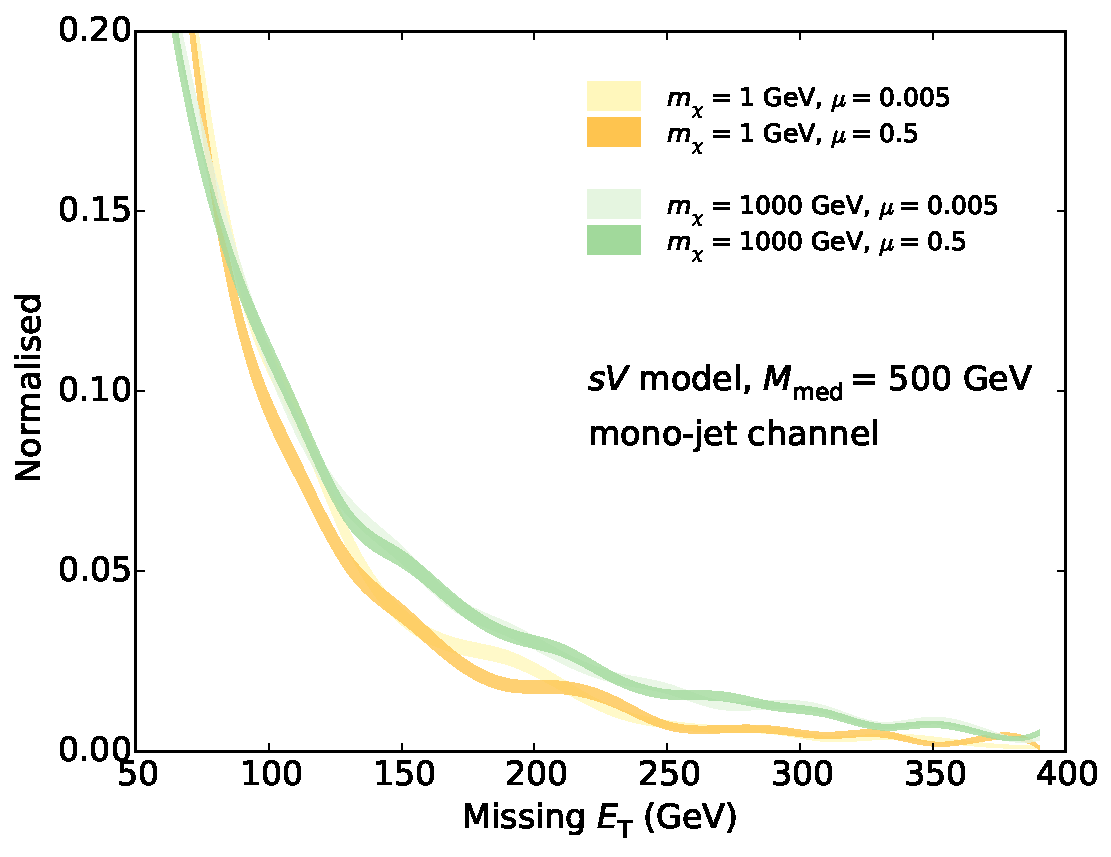
\includegraphics[width=0.495\textwidth]{figures/MET_monojet_SVD.pdf}
    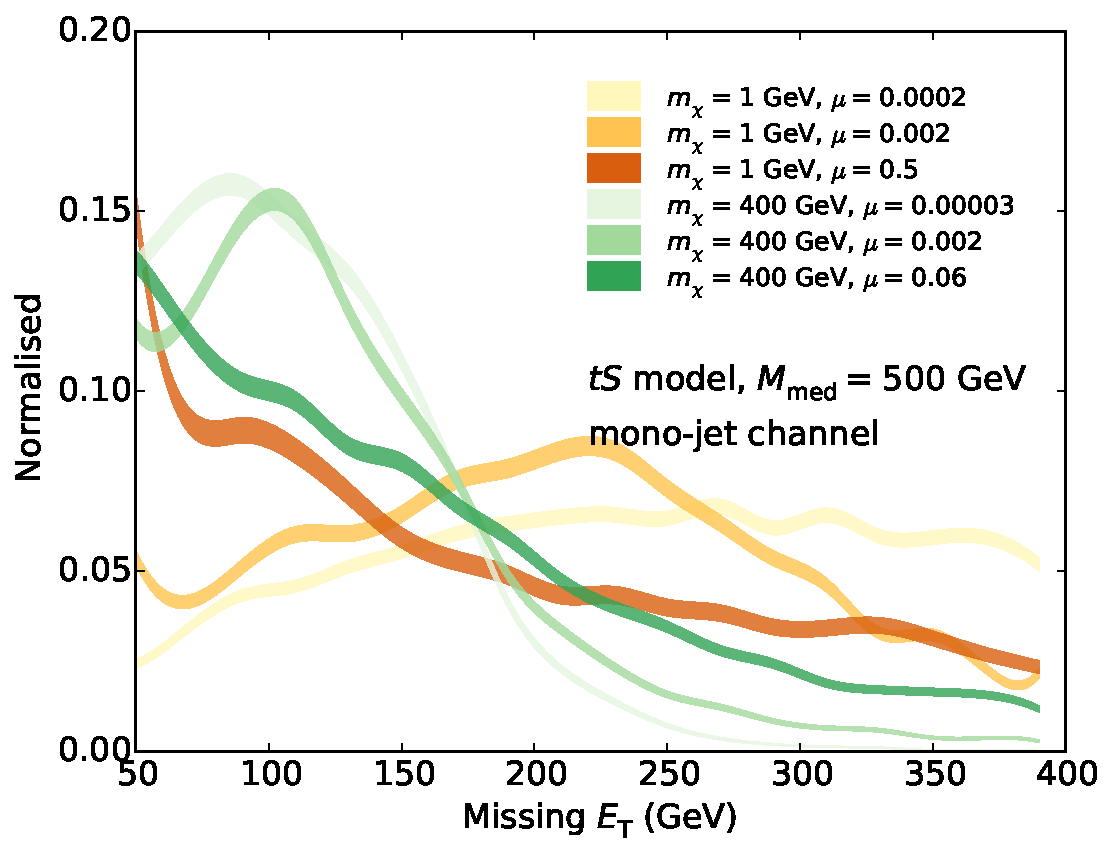
\includegraphics[width=0.495\textwidth]{figures/MET_monojet_TSD.pdf}
    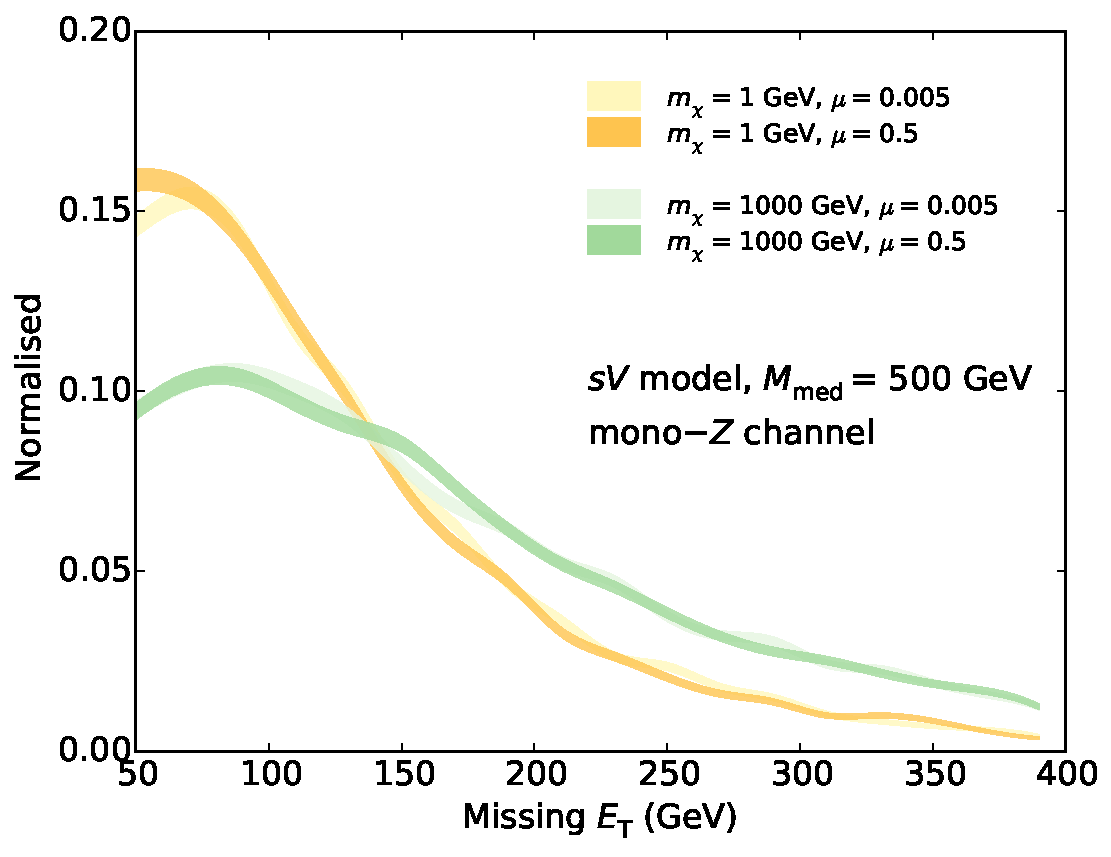
\includegraphics[width=0.495\textwidth]{figures/MET_monoZ_SVD.pdf}
    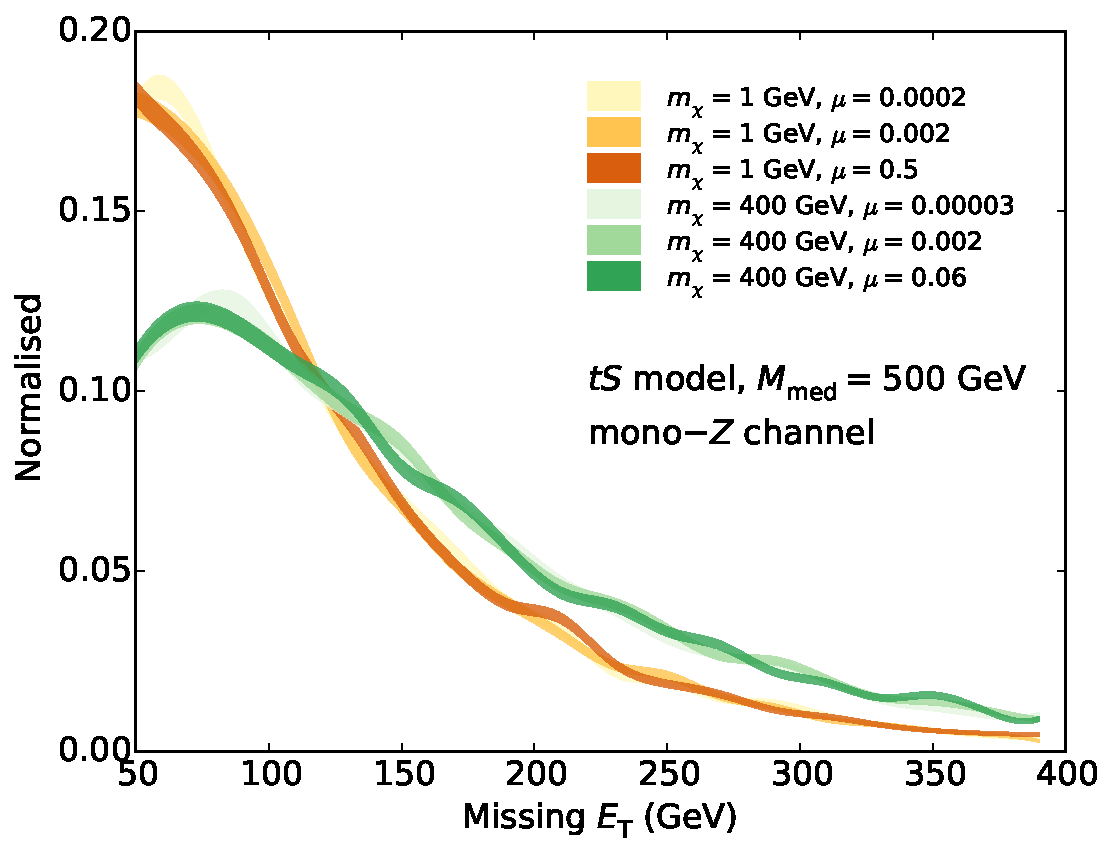
\includegraphics[width=0.495\textwidth]{figures/MET_monoZ_TSD.pdf}
    \caption{The $\met$ distribution of the $sV$ and $tS$ models in the \monojet and \monoZ channels, for some exemplary masses. The parameter $\mu$ is defined as $\Gamma / \Mmed$, and is used to demonstrate the impact of a changing width; the $tS$ model in the \monojet channel shows a clear width-dependence. The widths are obtained with couplings of 0.1, 1 and 5 where $\mu < 0.5$ remains true.}
    \label{fig:MET_dists}
  \end{center}
\end{figure}

%\textcolor{magenta}{This section should include:}
%\begin{enumerate}
%\item \textcolor{magenta}{Brief motivation for choice of simplified models? (eg. something like "we consider the most straightforward UV-completions of the D1, D5 and D8 effective operators, corresponding to the s-channel scalar, vector and axial-vector models respectively.}
%\item \textcolor{magenta}{The interaction Lagrangians for our four SiMs along with an explanation for why we only assume coupling to SM quarks.}
%\item \textcolor{magenta}{The assumptions and the decay widths associated with our models (?).}
%\item \textcolor{magenta}{Comments on the requirement that $\sqrtgqgX} \leq 4\pi$ in order for the theory to remain perturbative? $\rightarrow$ comments on the choice of mass and coupling points used? Or does this belong in section \ref{sec:sec3}?}
%\end{enumerate}

%Resolving the mediator leads to two possibilities: the mediating particle is exchanged in the s-channel, in which case it may be colour neutral, or it is exchanged in the t-channel in which case it is necessarily coloured \cite{}.

%\cite{ValidEFT, BeyondEFT, CSUSY} t-channel \cite{Buchmueller:2014yoa, SiM}.
